\chapter{Arquitectura}
\label{chap:arquitectura}

\drop{E}{}ste capítulo analiza en detalle, mediante un enfoque top-down, la arquitectura diseñada para dar soporte al sistema propuesto en este proyecto. Se discutirá la funcionalidad de cada módulo perteneciente a la arquitectura, se explicará cómo están conectados y cómo fluye la información entre ellos hasta obtener el resultado final. 

\section{Visión general de la arquitectura}
\label{sec:visiongeneral}

La arquitectura diseñada (ver Figura~\ref{fig:arquitectura}) es una arquitectura basada en módulos que contribuye a simplificar significativamente el desarrollo del sistema. 

\begin{figure}[!h]
\begin{center}
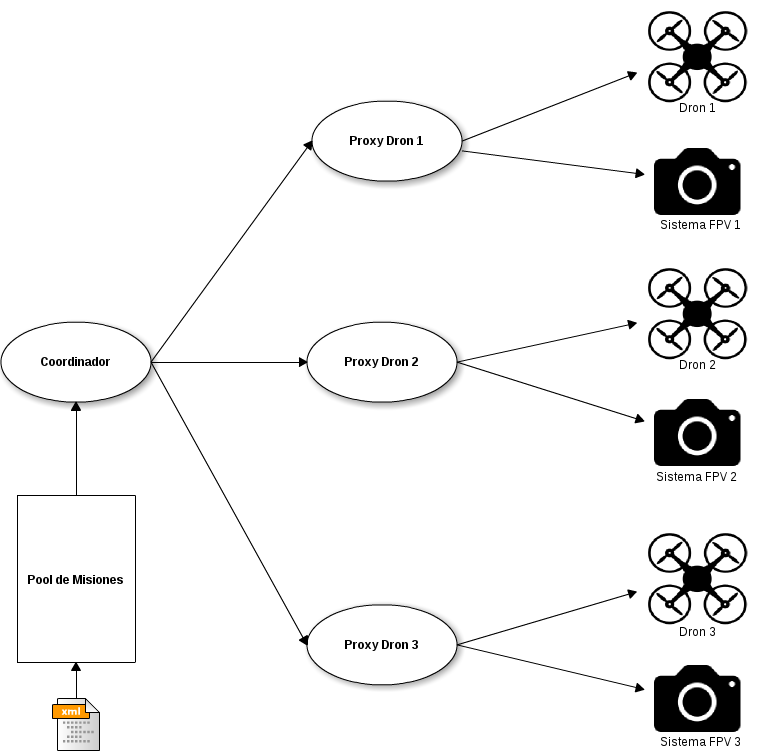
\includegraphics[width=0.8\textwidth]{/arquitectura.png}
\caption[Arquitectura del sistema]{Arquitectura del sistema}
\label{fig:arquitectura}
\end{center}
\end{figure}

La arquitectura modular se refiere al diseño de sistemas compuestos por elementos separados que pueden conectarse preservando relaciones proporcionales. La utilidad de la arquitectura modular se basa en la posibilidad de reemplazar o agregar cualquier componente sin afectar al resto del sistema.

Al aplicar la arquitectura modular, un problema complejo debe ser dividido en varios subproblemas más simples, y estos a su vez en otros subproblemas más simples. Esto debe hacerse hasta obtener subproblemas lo suficientemente simples como para poder ser resueltos fácilmente con algún lenguaje de programación.

Un módulo es cada una de las partes de un programa que resuelve uno de los subproblemas en que se divide el problema complejo original. Cada uno de estos módulos tiene una tarea bien definida y algunos necesitan de otros para poder operar. En caso de que un módulo necesite de otro, puede comunicarse con éste mediante una interfaz de comunicación que también debe estar bien definida. No debe confundirse el término módulo con términos como función o procedimiento, propios del lenguaje que lo soporte.

\begin{figure}[!h]
\begin{center}
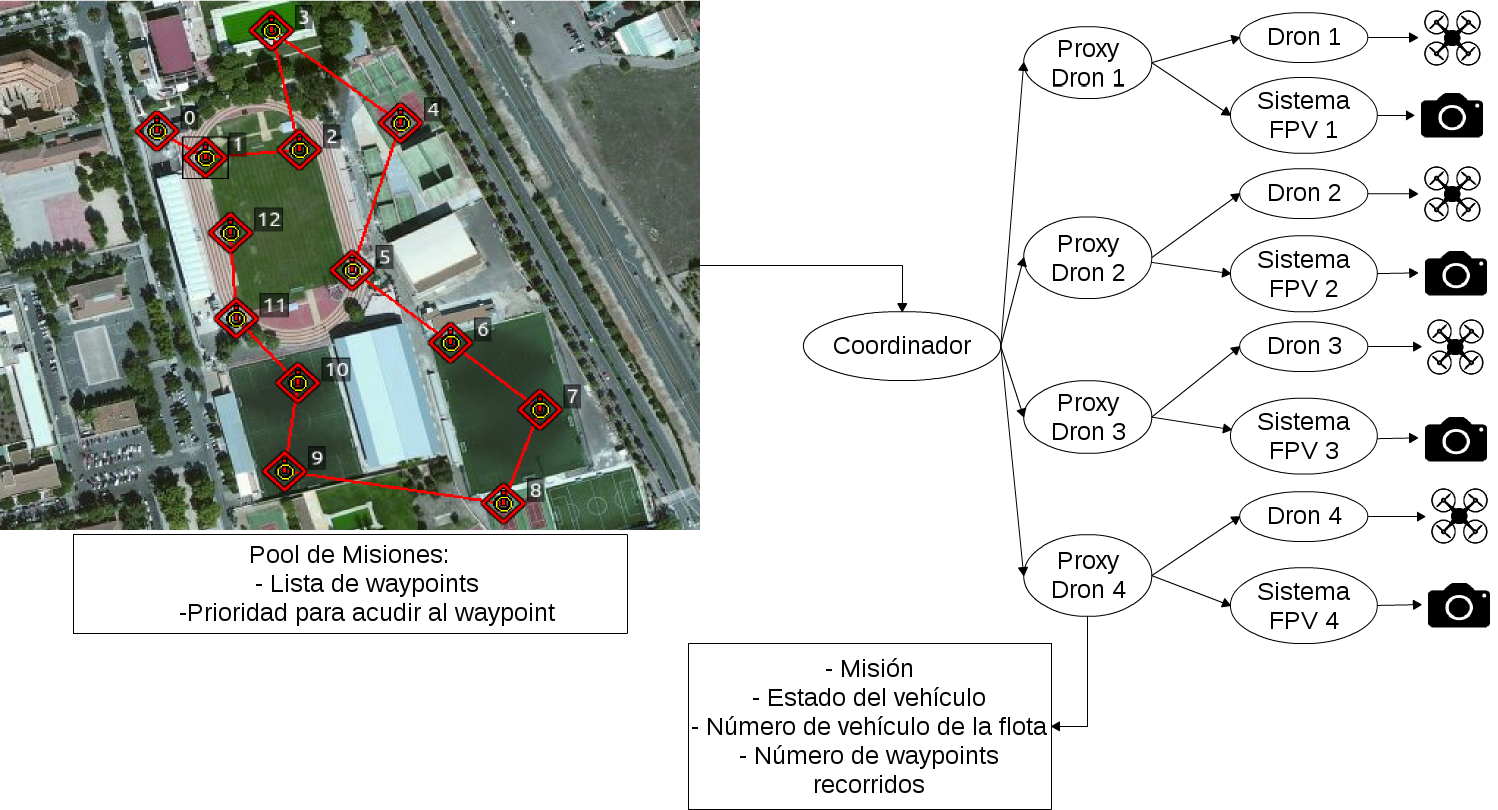
\includegraphics[width=0.8\textwidth]{/arquitectura2.png}
\caption[Descripción del sistema]{Descripción del sistema}
\label{fig:descripcion}
\end{center}
\end{figure}

La descripción de la arquitectura se elaborará a continuación atendiendo a las capas que forman el sistema.

\subsection{Capas de la arquitectura}
\label{sec:capas}

\subsubsection{Sistema operativo}
\label{sec:sistemaoperativo}

Un \textbf{sistema operativo} puede ser explicado como una suma de herramientas software que posibilitan al usuario la interacción con el computador. Un sistema operativo cuenta como mínimo con los siguientes elementos:

\begin{itemize}
\item \textbf{Núcleo}: es una serie de métodos y herramientas que proporcionan acceso a las funciones de bajo nivel para comunicarse con el hardware. 
\item \textbf{Drivers}: son librerías que permiten al sistema operativo trabajar con hardware concreto, como pueden ser tarjetas gráficas o impresoras. 
\item \textbf{Intérprete de comandos}: es una aplicación que posibilita al usuario la introducción de órdenes que son procesables por el computador. Suele realizarse mediante una línea de comandos.
\item \textbf{Biblioteca de llamadas al sistema}: métodos que propician que el software interactúe con el ordenador a través del sistema operativo.
\item \textbf{Editor de texto}: es un programa con el que se pueden crear, visualizar y modificar archivos de texto.
\item \textbf{Compilador}: transforma una sucesión de líneas de código, escritas en un lenguaje de programación específico, en un programa ejecutable.
\end{itemize} 

Estos elementos forman un conjunto muy simple. Los sistemas operativos actuales cuentan con numerosas herramientas adicionales, entre los que se encuentran los procesadores de texto, los entornos de desarrollo y los navegadores web. Adicionalmente, el usuario puede instalar software que sea compatible con el sistema operativo.

La función del sistema operativo en este proyecto es \textbf{facilitar el acceso al hardware} y aportar funcionalidades del sistema, como puede ser la comunicación entre procesos o el acceso a la red.

\subsubsection{Hardware}
\label{sec:hardwarearq}

Son las piezas físicas con las que se trabaja en última instancia, como pueden ser discos duros, tarjetas de red, memoria RAM, un dron o una cámara. Dado que el proyecto trata sobre drones en situaciones de catástrofe, el guiado, así como la comunicación con el dron, y el sistema \acs{FPV}, es una parte fundamental.

Su función en este proyecto es \textbf{comunicarse con la capa de abstracción hardware}, para así, poder hacer efectivas las instrucciones implementadas en el proyecto.

\subsubsection{Capa de abstracción hardware}
\label{sec:hardwareabs}

La \textbf{capa de abstracción de hardware} (\acs{HAL}) es un elemento del sistema operativo que funciona como una interfaz entre el software y el hardware del sistema, proveyendo una plataforma de hardware consistente sobre la cual corren las aplicaciones. 

Cuando se emplea una capa de abstracción de hardware, las aplicaciones no acceden directamente al hardware sino que lo hacen a la capa abstracta provista por la \acs{HAL}. Del mismo modo que una \acs{API}, la HAL permite que las aplicaciones sean independientes del hardware porque abstraen información acerca de tales sistemas, como lo son las cachés, los buses de E/S y las interrupciones, y usan estos datos para darle al software una forma de interactuar con los requerimientos específicos del hardware sobre el que deba correr.

La \acs{HAL} permite que las aplicaciones puedan extraer tanto rendimiento como sea posible del hardware; proporciona acceso directo a cada dispositivo hardware; permite que el software se comunique con el hardware a nivel general y facilita la portabilidad.

Su función en este proyecto es \textbf{hacer que se lleven a cabo las instrucciones de los procesos que lo componen} como pueden ser: el almacenamiento de imágenes y videos, la transmisión de órdenes al dron a través de la interfaz USB, la transmisión de imágenes a través de la red, etc.

\subsubsection{Framework}
\label{sec:framework}

Un \textbf{framework} es una estructura conceptual y tecnológica de soporte definido, normalmente con artefactos o módulos concretos de software, que puede servir de base para la organización y desarrollo de software.

En este caso, es el proyecto propuesto, el cual consiste en un sistema de vigilancia adaptativo basado en la coordinación de \acs{UAV}s. Proporciona un conjunto de \textbf{servicios, funciones y herramientas} como puede ser el uso de una estación de control de tierra, la lectura de «waypoints», la ordenación de estos por prioridad, el vuelo de un vehículo aéreo o la grabación y el análisis de imágenes.

\subsubsection{Módulos desarrollados}
\label{sec:modulos}

Los \textbf{módulos} que se han desarrollado son las unidades básicas que el framework es capaz de manejar y de las que depende la solución que se implemente con él. El sistema está compuesto por los siguientes módulos:

\begin{itemize}
\item \textbf{Módulo de Interpretación de Misiones}: en él se interpretan los archivos XML que contienen las referencias de puntos de localización y posteriormente se ordenan esas localizaciones por la prioridad de acudir a cada una de ellas.
\item \textbf{Módulo de Coordinación}: se coordina la actividad de los drones para mejorar la productividad del sistema. Asigna misiones a vehículos que no estén ejecutando algún vuelo hacia algún «waypoint». Además, ordena el aterrizaje cuando en el \textit{Módulo de Interpretación de Misiones} no queden misiones por asignar.
\item \textbf{Módulo de Despliegue de Alto Nivel}: es el módulo que se conecta y comunica con el vehículo, de modo que, actúa como mediador entre el \textit{Módulo de Coordinación} y el \textit{Módulo de Despliegue de Bajo Nivel}. Permite efectuar tareas relacionadas con el dron, así como administrar la conexión con el \textit{Módulo de Análisis de Información}.
\item \textbf{Módulo de Despliegue de Bajo Nivel}: se encarga de crear una simulación de un dron, en una localización específica, para poder realizar pruebas, misiones o cualquier tipo de operación que se podría llevar a cabo con un dron real.
\item \textbf{Módulo de Análisis de Información}: captura, graba y almacena imágenes, en \acs{FPV}, del vuelo del vehículo. Las imágenes son analizadas por una \acs{API} externa de Google, Google Cloud Vision \acs{API}, que detecta conjuntos de categorías y devuelve una serie de resultados después de realizar una petición \acs{HTTP}. 
\end{itemize} 

\subsubsection{Clases}
\label{sec:clases}

Cada módulo representa una o más clases en las que se define el comportamiento mediante atributos y funciones. Las clases son instanciadas en objetos, que se corresponden tanto con objetos reales como con objetos internos del sistema, en los que se leen estas definiciones.

\begin{itemize}
\item \textbf{Coordinador}: realiza una lectura del \textit{Pool de misiones} ordenándolo por prioridad, se encarga de crear instancias del objeto \textit{ProxyDrone}, asignar «waypoints» a vehículos desocupados y ordenar el aterrizaje cuando el \textit{Pool de misiones} este vacío. El \textit{Coordinador} forma parte del \textit{Módulo de Interpretación de Misiones} y del \textit{Módulo de Coordinación}.
\item \textbf{Proxy Dron}: es el responsable a la hora de realizar las operaciones que conciernen al vehículo, como el despegue o la subida de misiones, y de gestionar la conexión con los dispositivos finales, como el \textit{dron} o el \textit{sistema \acs{FPV}}. El \textit{Proxy Dron} forma parte del \textit{Módulo de Coordinación} y del \textit{Módulo de Despliegue de Alto Nivel}.
\item \textbf{Dron}: Crea una simulación de un vehículo aéreo no tripulado en una localización determinada. El \textit{Dron} forma parte del \textit{Módulo de Despliegue de Bajo Nivel}.
\item \textbf{Sistema \acs{FPV}}: Captura imágenes en vivo, las analiza y muestra en pantalla los resultados. El \textit{Sistema \acs{FPV}} forma parte del \textit{Módulo de Análisis de Información}.
\end{itemize}

Estas clases, junto a sus funciones, serán explicadas en detalle en las siguientes secciones de este capítulo. 

En el sistema la información fluye a través de las clases (ver Figura~\ref{fig:diagflujo}), transformándose hasta alcanzar el resultado final. Esto es, los vehículos aéreos se desplazan de manera coordinada a diversas localizaciones y a su vez retransmiten imágenes, que son analizadas para contribuir a mejorar los tiempos de respuesta en situaciones de emergencia.

\begin{figure}[!h]
\begin{center}
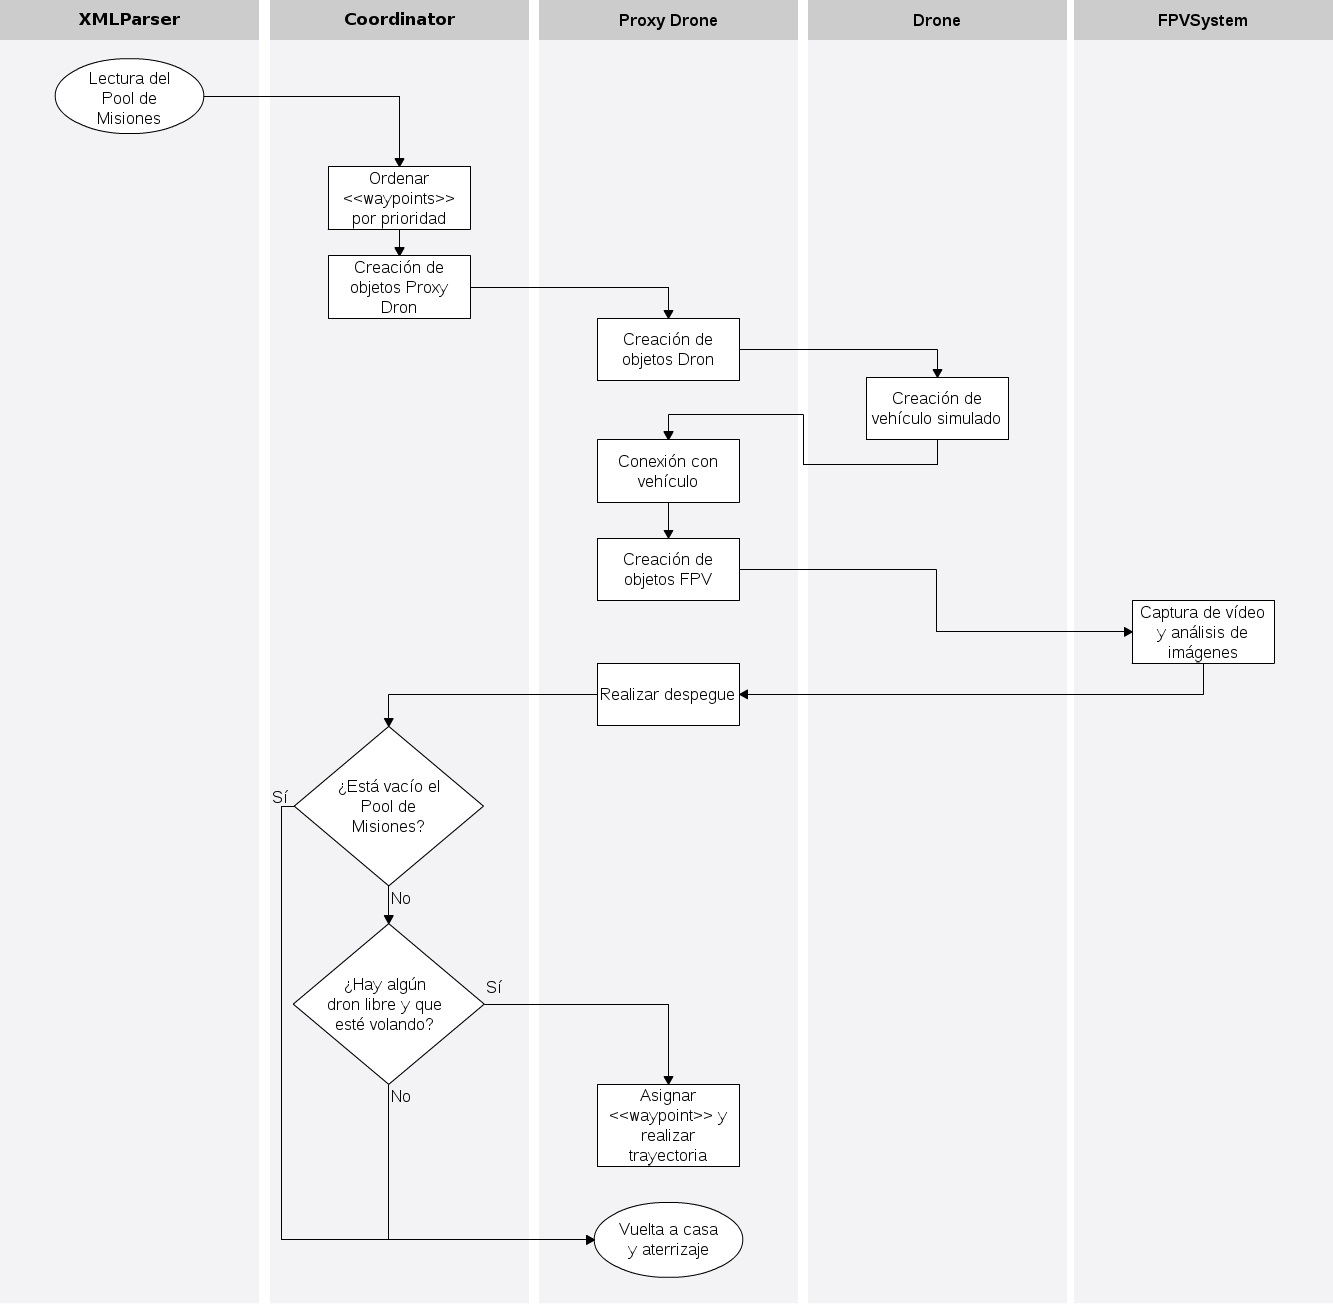
\includegraphics[width=1\textwidth]{/Flowchart.png}
\caption[Diagrama de flujo del sistema con un solo dron]{Diagrama de flujo del sistema con \textbf{un solo dron}}
\label{fig:diagflujo}
\end{center}
\end{figure}

\clearpage

\subsection{Coordinador}
\label{sec:coordinador}

El \textbf{\textit{Coordinador}} es el responsable de llevar a cabo la \textbf{coordinación} (ver Figura~\ref{fig:diagclases}), \textbf{entre los \acs{UAV}s} que existan disponibles, con el objetivo de poder abarcar el mayor terreno posible en un tiempo que es considerablemente menor. En resumen, su cometido consiste en \textbf{asignar puntos de interés} a drones que se encuentren \textit{en vuelo} y en un \textit{estado ocioso}. 

\begin{figure}[!h]
\begin{center}
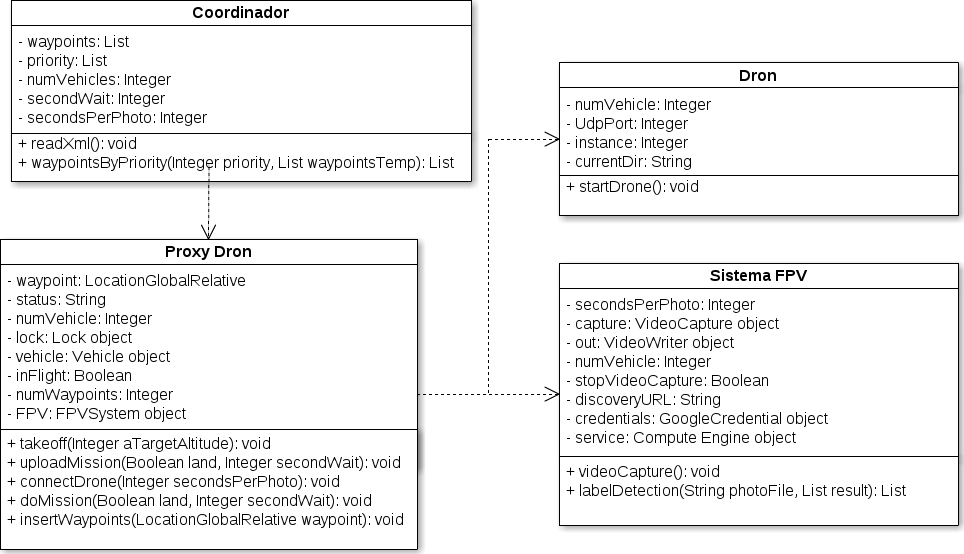
\includegraphics[width=0.8\textwidth]{/clases_completo.png}
\caption[Diagrama de clases del sistema]{Diagrama de clases del sistema}
\label{fig:diagclases}
\end{center}
\end{figure}

Para cumplir con su función el \textit{Coordinador} debe:

\begin{itemize}
\item \textbf{Leer el \textit{Pool de Misiones}}: el sistema se vale de \textbf{archivos XML} (ver Listado~\ref{code:archivoxml}) que contienen la información acerca de los puntos de interés a los que los drones deben acudir: \textbf{longitud}, \textbf{latitud}, \textbf{altura} a la que el dron debe volar en dicha posición y la \textbf{prioridad} de que el \acs{UAV} vuele hasta esa localización. La lectura de estos archivos XML ocasiona la \textbf{creación} de una estructura de tipo lista, que denominaremos \textbf{\textit{Pool de Misiones}}, que contiene una serie de puntos de interés. 
\item \textbf{Ordenar \textit{Pool de Misiones} por prioridad}: una vez que los archivos XML han sido leídos y los «waypoints» han sido almacenados en el \textit{Pool de Misiones}, el \textit{Coordinador} debe \textbf{ordenar} esas localizaciones \textbf{por medio del campo prioridad}. La prioridad puede tomar tres valores diferentes: 1, 2 y 3. Siendo 1 la prioridad más elevada y 3 la de menor relevancia. De modo que, en el \textit{Pool de Misiones} deben aparecer primero los «waypoints» cuya prioridad sea de 1 y en último lugar los que tengan una prioridad de 3, consiguiendo que los drones lleguen antes a los puntos de interés más importantes.
\item \textbf{Asignar «waypoints»}: las localizaciones son \textbf{adjudicadas}, hasta vaciar el \textit{Pool de Misiones}, a drones que se encuentren \textbf{\textit{en vuelo}} y que se hallen \textbf{en un \textit{estado ocioso}}, es decir, a drones que ya hayan realizado el despegue y, además, hayan terminado de volar hacia un punto de interés en el que han recogido las imágenes especificadas. 
\item \textbf{Ordenar el aterrizaje}: cuando el \textit{Pool de Misiones} ha sido vaciado, el \textit{Coordinador} ordena la vuelta a casa y el aterrizaje de cada uno de los drones que se estaban empleando en el proceso.
\end{itemize}

\begin{listing}[
 float=,
 language = XML,
 caption = {Ejemplo de archivo XML que contiene la información de los «waypoints»},
 label  = code:archivoxml]
<?xml version="1.0" ?>
<mission>
	<waypoint>
 		<long>32.8353314496671587</long>
 		<lat>-117.162768244743347</lat>
		<alt>20</alt>
		<priority>2</priority>
	</waypoint>

	<waypoint>
 		<long>32.8353359570248671</long>
 		<lat>-117.161904573440552</lat>
		<alt>40</alt>
		<priority>1</priority>
	</waypoint>

	<waypoint>
 		<long>32.8353359570248671</long>
 		<lat>-117.161904573440552</lat>
		<alt>10</alt>
		<priority>3</priority>
	</waypoint>
</mission>
\end{listing}


Es crucial que varios drones puedan \textbf{efectuar a la vez el vuelo y la captura de vídeo}, por lo que es necesario la \textbf{introducción de hilos} en el \textit{Coordinador}, que permitan ejecutar, de manera paralela, estas funciones. 

La técnica de multi-hilos permite \textbf{desacoplar tareas que no tienen dependencia secuencial}, pudiendo ser usada para mejorar el grado de reacción de las aplicaciones que aceptan entradas del usuario mientras otras tareas se ejecutan en segundo plano. El trabajo con threads se lleva a cabo mediante el \textbf{módulo \textit{threading}} que se apoya en el módulo \textit{thread} para proporcionar una \acs{API} de más alto nivel, más completa y orientada a objetos. 

El desafío principal de las aplicaciones multi-hilo es la coordinación entre los hilos que comparten datos u otros recursos. Con ese fin, el módulo \textit{threading} provee una serie de primitivas de sincronización que incluyen \textbf{\textit{locks}}, eventos, variables de condición y semáforos. 

Los \textit{locks}, también llamados mutex, cierres de exclusión mutua, cierres o candados, son objetos con \textbf{dos estados posibles: adquirido o libre}. Cuando un \textit{thread} adquiere el candado, los demás \textit{thread} que lleguen a ese punto posteriormente y pidan adquirirlo se bloquearán hasta que el \textit{thread} que lo ha adquirido libere el candado, momento en el cual podrá entrar otro \textit{thread}.

El \textit{Coordinador} está compuesto por atributos y métodos (ver Figura~\ref{fig:diagclasescoord}) necesarios para llevar a cabo la \textbf{coordinación de los drones}.

\begin{figure}[!h]
\begin{center}
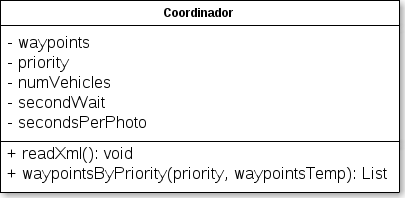
\includegraphics[width=0.8\textwidth]{/clases_coordinador.png}
\caption[Diagrama de clases del \textit{Coordinador}]{Diagrama de clases del \textit{Coordinador}}
\label{fig:diagclasescoord}
\end{center}
\end{figure}

Para iniciar el sistema, se debe realizar una llamada a la clase \textbf{\textit{Coordinador}}, la cual cuenta con tres argumentos que son parametrizables al realizar su invocación por consola. Estos atributos parametrizables son los siguientes:
\begin{itemize}
\item \textbf{numVehicles}: se refiere al número de vehículos que participarán en las misiones y capturarán imágenes en directo del vuelo. Si se omite, el valor por defecto es 1 vehículo.
\item \textbf{secondWait}: afecta al número de segundos que el vehículo permanecerá parado sobre un «waypoint» para captar imágenes relevantes de esa localización durante ese tiempo. Si se omite, el valor por defecto es de 10 segundos.
\item \textbf{secondsPerPhoto}: referido al número de segundos que deben transcurrir para tomar una fotografía. Por ejemplo, si el valor es de 5 segundos, el sistema realizará una fotografía cada 5 segundos. Si se omite, el valor por defecto es de 10 segundos.
\end{itemize} 

Un ejemplo de cómo realizar la llamada a \textit{Coordinador} puede ser:

\begin{listing}[
 float=h!,
 language = bash,
 caption = {Ejemplo de llamada a \textit{Coordinador}},
 label  = code:coordinador]
$ python coordinator.py --vehicles 2 --secondWait 15 --secondsPerPhoto 7
\end{listing}


\subsection{Proxy Dron}
\label{sec:proxydron}

El \textbf{\textit{Proxy Dron}} es el encargado de ejecutar las tareas que tienen que ver con el \acs{UAV} y de administrar la conexión con los dispositivos finales. Se puede considerar un \textbf{intermediario} entre el \textit{Coordinador} y los instrumentos que se encuentran en el extremo del sistema, \textit{Dron} y \textit{Sistema \acs{FPV}}, que son usados para realizar el vuelo y captar imágenes.

Mediante el \textit{Proxy Dron} se resuelve el problema de \textbf{guiar el vehículo} a través de una serie de puntos de localización. Gracias a él, el sistema cuenta con una clase que posibilita la \textbf{comunicación con el dron} y con el \textbf{sistema de visionado en primera persona}, permitiendo así realizar cualquier tipo de operación como el despegue, la asignación de puntos de interés, la realización de vuelos a dichos puntos o la captación de imágenes que puedan ayudar al personal de emergencia en las labores de identificación de supervivientes o inspección del terreno.

Tan pronto como se haya realizado la lectura de los archivos XML y se cuente con una lista de «waypoints» ordenados por prioridad, se procede a crear objetos de tipo \textbf{\textit{Proxy Dron}} (ver Figura~\ref{fig:diagclasesproxy}). 
%Para ello, el \textit{Coordinador} hace uso de su atributo \textit{numVehicles}, creando tantos objetos \textit{Proxy Dron} como número de vehículos se haya especificado.

\begin{figure}[!h]
\begin{center}
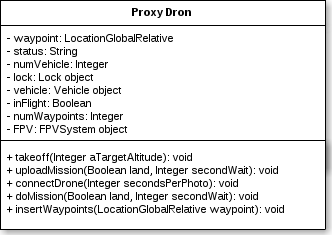
\includegraphics[width=0.8\textwidth]{/clases_proxydron.png}
\caption[Diagrama de clases del \textit{Proxy Dron}]{Diagrama de clases del \textit{Proxy Dron}}
\label{fig:diagclasesproxy}
\end{center}
\end{figure}

Entre las competencias de este objeto se encuentran las que se exponen a continuación:

\begin{itemize}
\item \textbf{Conexión con el dron} y con el \textbf{Sistema \acs{FPV}}: En el caso de ejecutar una simulación del sistema, se instancia un objeto de tipo \textit{Dron}, que creará un vehículo simulado mediante \acs{SITL} (véase Sección \ref{sec:sitl}). A continuación, se realiza la conexión con el vehículo aéreo, ya sea real o simulado, y por último se crea un objeto \textit{Sistema \acs{FPV}} para iniciar la grabación y el análisis de imágenes.
\item \textbf{Despegue} del dron: se comprueba que el vehículo cumpla ciertos requisitos antes de armar los motores, como que disponga de una buena señal de \acs{GPS} o que el nivel de la batería sea superior al 50\%, se configura el modo de pilotaje del dron y se procede al despegue a una altura especificada por parámetro. Cuando el despegue ha terminado, el dron se considera \textit{en vuelo}. 
\item \textbf{Inserción de «waypoints»} y \textbf{escritura de misiones}: los «waypoints», que han sido extraídos del archivo XML en el \textit{Coordinador}, son adjudicados a drones que se encuentren en \textit{estado ocioso} y \textit{en vuelo}. La localización de estos puntos debe ser agregada a comandos de misión que puedan ser interpretados por el vehículo. Entre estos comandos se encuentran las órdenes necesarias para: acudir a una localización específica, mantener el vehículo en un punto concreto o realizar la vuelta a casa y el aterrizaje.
\end{itemize}

El \textit{Proxy Dron} es inicializado pasándole por parámetro el número de vehículo con el que se corresponde dicho objeto. Gracias a esto, el usuario puede obtener \textbf{información del estado del dron}, sabiendo, por ejemplo, si esa información está asociada al \textit{Dron 1} o al \textit{Dron 2}. Es el responsable de llevar a cabo las \textbf{operaciones de vuelo} y de \textbf{administrar la conexión con los dispositivos finales}.

\subsection{Dron}
\label{sec:dron}

La clase \textbf{\textit{Dron}} ofrece la posibilidad de \textbf{simular vehículos aéreos} (ver Figura~\ref{fig:dronSITL}), en el caso de este proyecto un quadcopter, haciendo uso de la aplicación \acs{SITL}.

\begin{figure}[!h]
\begin{center}
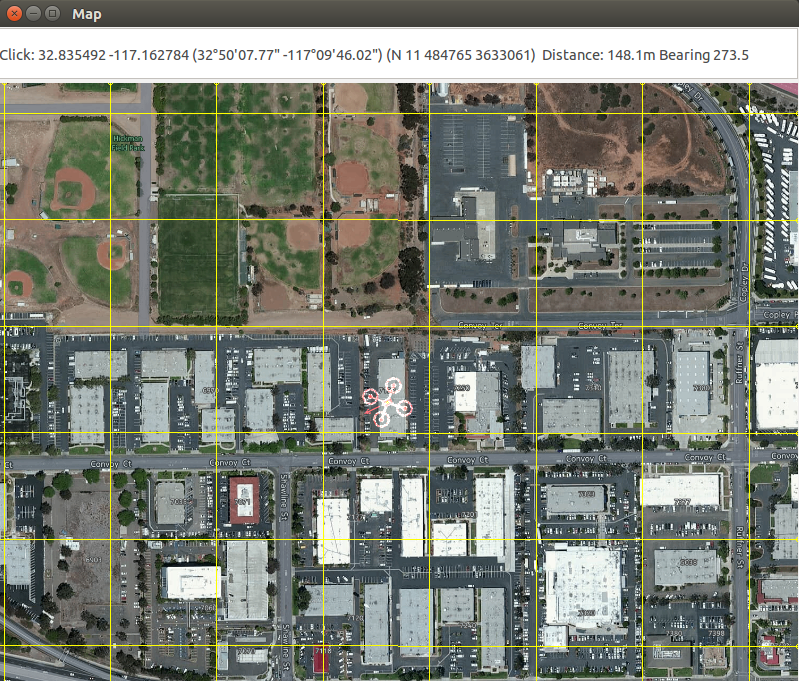
\includegraphics[width=0.8\textwidth]{/dronSITL.png}
\caption[Simulación de dron mediante \acs{SITL}]{Simulación de dron mediante \acs{SITL}}
\label{fig:dronSITL}
\end{center}
\end{figure}

El uso de \acs{SITL} (véase Sección \ref{sec:sitl}) es como usar un vehículo real: se puede conectar al vehículo usando una estación de control de tierra, despegar, cambiar los modos de vuelo, realizar misiones guiadas o automáticas, y aterrizar. La diferencia principal es que además de ser capaz de configurar el vehículo, los parámetros del simulador permiten configurar el entorno físico (por ejemplo, la velocidad y dirección del viento) y también simular el fallo de distintos componentes. Esto significa que \acs{SITL} es el entorno perfecto para probar correcciones de errores y otros cambios en el piloto automático, modos de fallo y aplicaciones desarrolladas mediante DroneKit-Python (véase Sección \ref{sec:dronekit}).

El cometido que tiene este objeto es, dependiendo del número de vehículo que lo instancie, acceder a una carpeta determinada y \textbf{ejecutar el comando} (ver Listado~\ref{code:simulacion}) \textbf{para generar la simulación} del dron, en un puerto UDP concreto, al que posteriormente el sistema se conectará para comunicarse con él.

\begin{figure}[!h]
\begin{center}
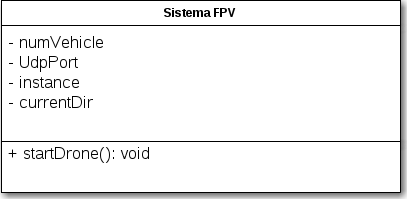
\includegraphics[width=0.8\textwidth]{/clases_dron.png}
\caption[Diagrama de clases del \textit{Dron}]{Diagrama de clases del \textit{Dron}}
\label{fig:diagclasesdron}
\end{center}
\end{figure}

\begin{listing}[
 float=h!,
 language = bash,
 caption = {Comando para generar una simulación de un vehículo mediante \acs{SITL}},
 label  = code:simulacion]
$ sim_vehicle.sh -I %d -L prueba --map --out 127.0.0.1:%d --aircraft test
\end{listing}

El comando está formado por unos parámetros que representan lo siguiente:
\begin{itemize}
\item \textbf{-I}: el número de instancia para permitir múltiples copias del simulador funcionando a la vez.
\item \textbf{-L}: ubicación inicial, que es configurada en un archivo de tipo texto denominado \textit{locations.txt}.
\item \textbf{$-$$-$map}: posibilita disponer de una ventana con un mapa, para mostrar el progreso del dron al realizar las misiones.
\item \textbf{$-$$-$out}: dirección en la que se podrá realizar la conexión con el dron. Está formada por una dirección IP y un puerto UDP. \\ \\
\end{itemize}

\subsection{Sistema \acs{FPV}}
\label{sec:sistemafpv}

Los objetos de la clase \textbf{\textit{Sistema \acs{FPV}}} (ver Figura~\ref{fig:diagclasesfpv}) facilitan la captura de imágenes en \acs{FPV} y el análisis de estas.

\begin{figure}[!h]
\begin{center}
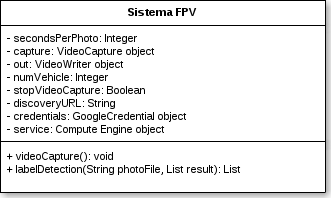
\includegraphics[width=0.8\textwidth]{/clases_fpv.png}
\caption[Diagrama de clases del \textit{Sistema \acs{FPV}}]{Diagrama de clases del \textit{Sistema \acs{FPV}}}
\label{fig:diagclasesfpv}
\end{center}
\end{figure}

Las tareas que se desarrollan en esta clase son fundamentalmente tres:
\begin{itemize}
\item \textbf{Grabación de vídeo}: el sistema graba y almacena un vídeo, haciendo uso de OpenCV (véase Sección \ref{sec:opencv}), que facilitará a los equipos de emergencia la visión del terreno, para así, poder tomar unas decisiones mejores y más correctas.
\item Realización de \textbf{captura de pantalla}: cada un cierto número de segundos, especificado al realizar la llamada al \textit{Coordinador}, se llevará a cabo una captura de pantalla que será almacenada en el computador y que será utilizada para realizar el análisis.
\item \textbf{Análisis de imágenes}: haciendo uso de Google Cloud Vision \acs{API} (véase Sección \ref{sec:visionapi}) se analizarán las capturas de pantalla realizadas anteriormente. Google Cloud Vision \acs{API}, mediante la detección de etiquetas, detecta amplios conjuntos de categorías y arroja resultados de los elementos que se encuentran dentro de las fotografías. Estos resultados serán imprimidos y mostrados en el vídeo que se está grabando. \\
\end{itemize}

Para llevar a cabo el análisis de imágenes es necesario realizar una \textbf{petición \acs{HTTP} a Google Cloud Vision \acs{API}} en la que se especifique el tipo de análisis que se quiere realizar, en este supuesto \textit{Detección de etiquetas}, y el número máximo de resultados que se quieren obtener. \\ \\

Un ejemplo de esta petición puede ser la especificada a continuación:

\begin{listing}[
 float=h!,
 language = Python,
 caption = {Ejemplo de petición a Google Cloud Vision \acs{API} para la detección de etiquetas},
 label  = code:analisis]
with open(photoFile, 'rb') as image:
	image_content = base64.b64encode(image.read())
    service_request = self.service.images().annotate(body = {
    	'requests': [{
        	'image': {
          		'content': image_content.decode('UTF-8')
        			},
        		'features': [{
          			'type': 'LABEL_DETECTION',
          			'maxResults': 5
        		}]
      	}]
    }]
    
		
    response = service_request.execute()
	responseLength = len(response['responses'][0])
\end{listing}

Haciendo uso de dicha función, se obtiene el análisis de una imagen que arroja como resultado cinco etiquetas.  

\begin{figure}[!h]
\begin{center}
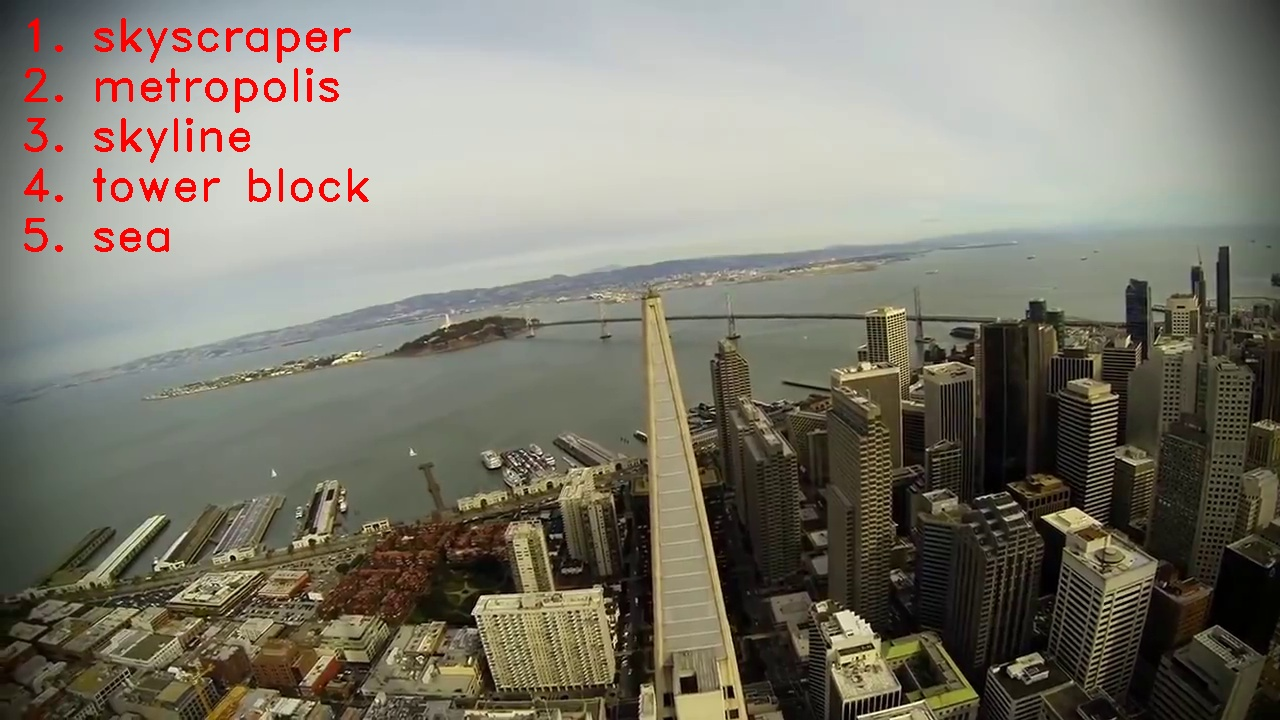
\includegraphics[width=0.8\textwidth]{/ejemplofpv.jpg}
\caption[Ejemplo de captura y análisis de imagen]{Ejemplo de captura y análisis de imagen}
\label{fig:ejemplofpv}
\end{center}
\end{figure}

% Local Variables:
% coding: utf-8
% mode: latex
% mode: flyspell
% ispell-local-dictionary: "castellano8"
% End:
